\documentclass{article}

\usepackage{graphicx}
\usepackage{tikz}
\usepackage{tikzsymbols}
\usetikzlibrary{calc,patterns,shapes.geometric}
\pagestyle{empty}
\usepackage[margin=0pt]{geometry}
\geometry{papersize={14in,12in}}

\def\centerarc[#1](#2)(#3:#4:#5){\draw[#1] ($(#2)+({#5*cos(#3)},{#5*sin(#3)})$) arc (#3:#4:#5);}

\begin{document}
	\begin{figure}
		\centering
		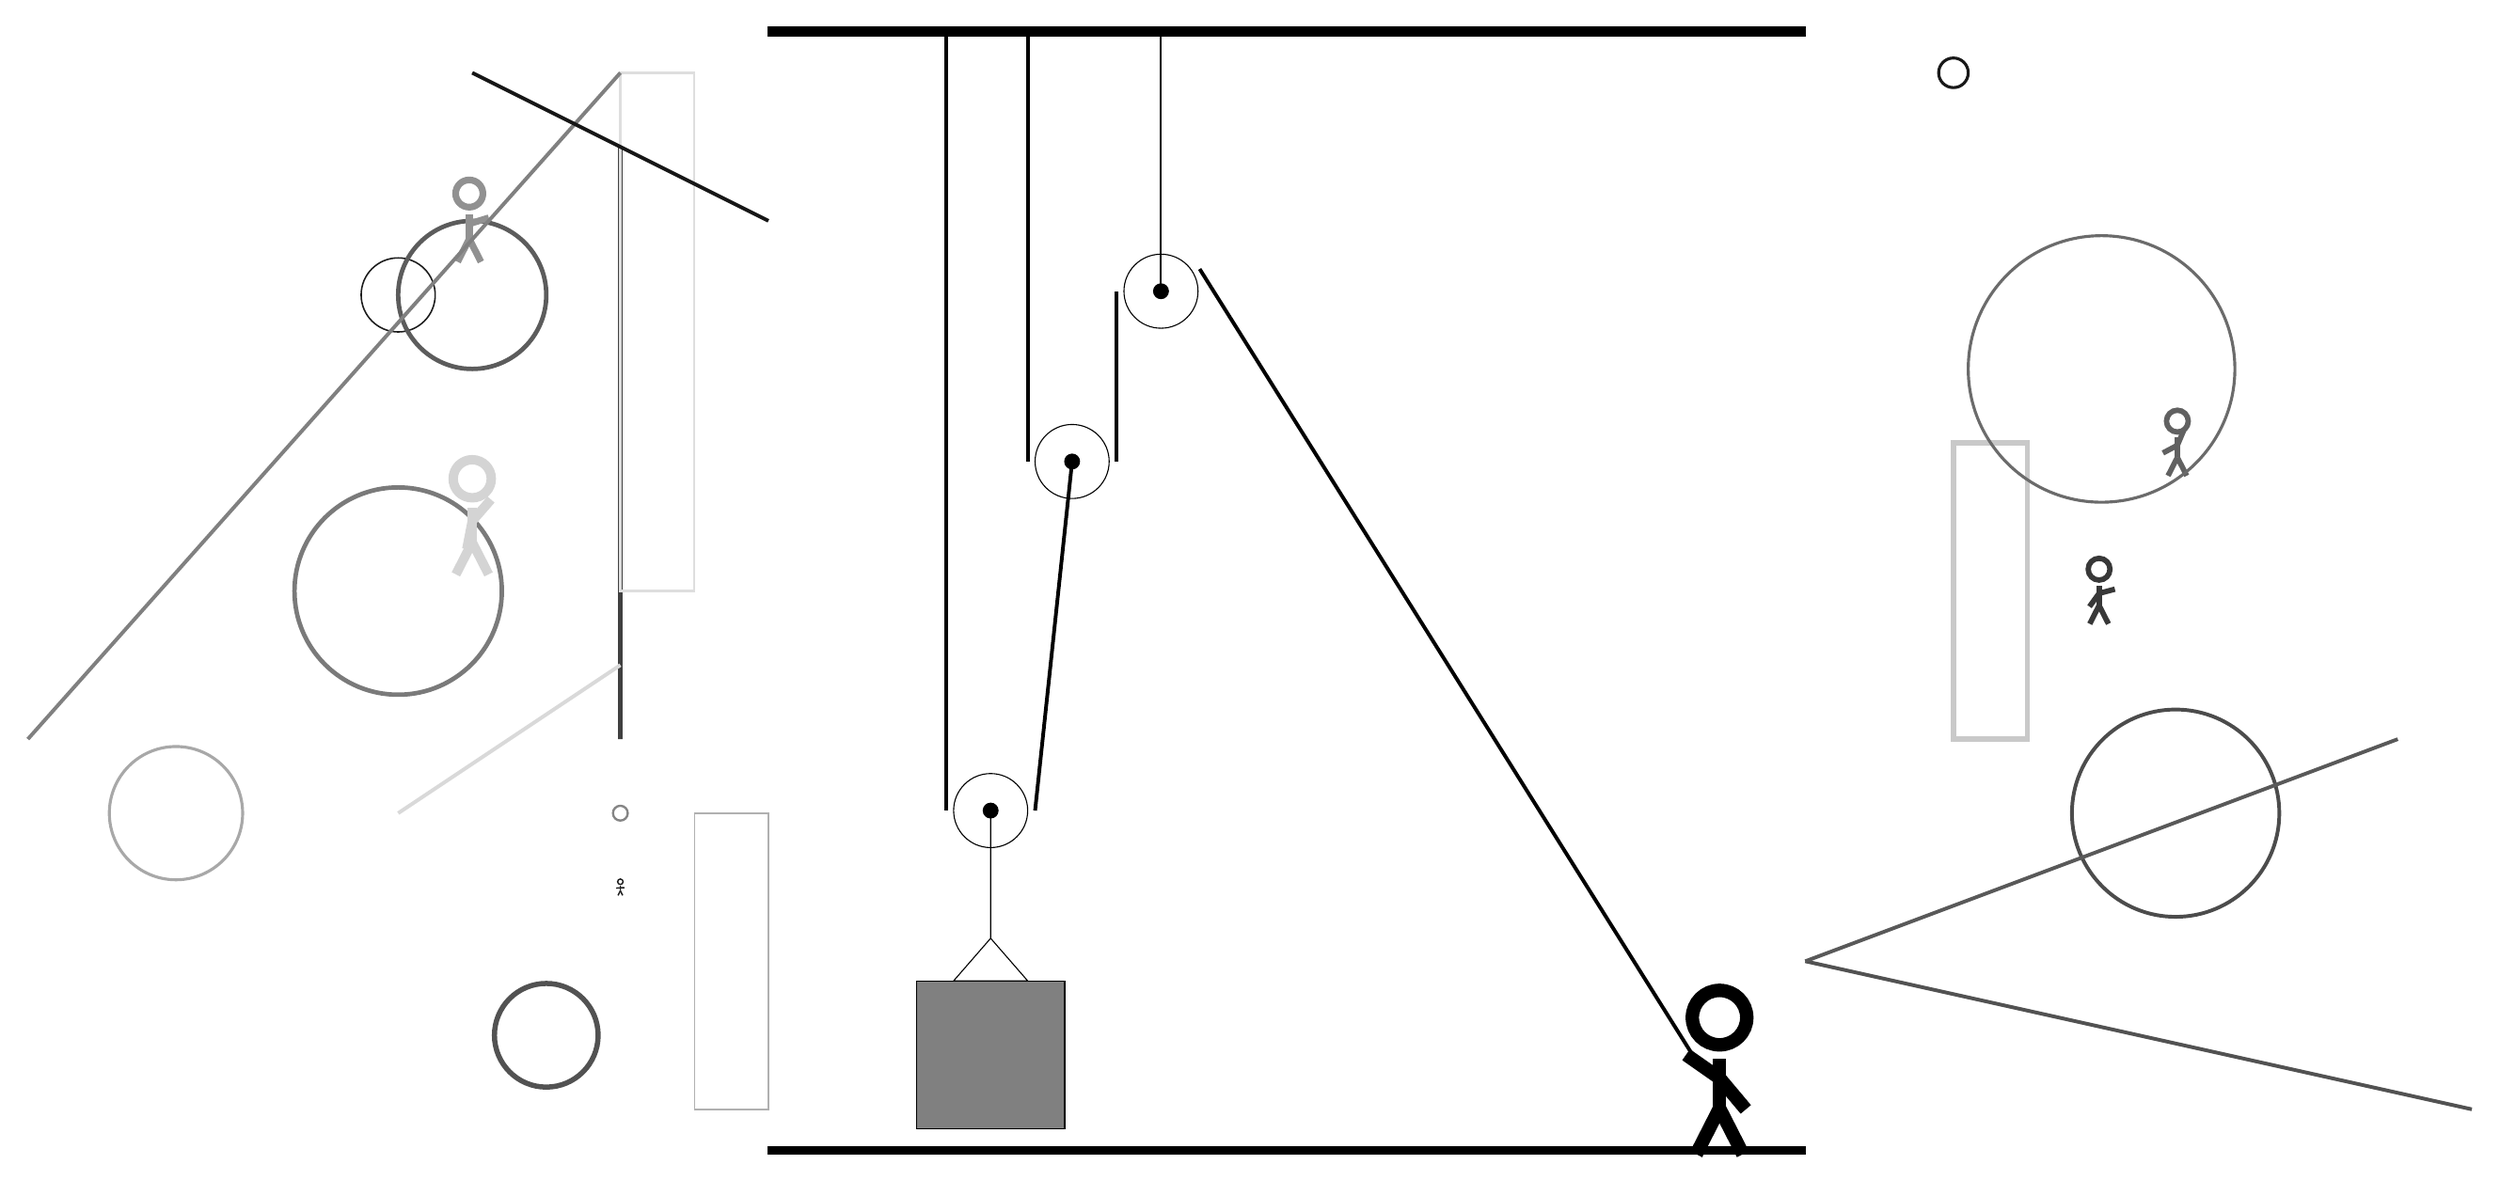
\begin{tikzpicture}
			%%%%% START %%%%%
			
			\draw[fill=black] (-2, 11.5) rectangle (12, 11.625);
			
			\draw (1, 1.035) circle (0.5);
			\draw[fill=black] (1, 1.035) circle (0.1);
			
			\draw (2.1, 5.75) circle (0.5);
			\draw[fill=black] (2.1, 5.75) circle (0.1);
			
			\draw [line width=0.2mm, color=black!89](-7, 8) circle (0.5);
			
			\draw [line width=0.7mm, color=black!68](-5, -2) circle (0.7);
			\draw [line width=0.6mm, color=black!64](-6, 8) circle (1.0);
			\draw[line width=0.2mm, color=black!31] (-3, -3) rectangle (-2, 1);
			\draw[line width=0.6mm, color=black!75] (-4, 10) rectangle (-4, 2);
			\draw[line width=0.3mm, color=black!13] (-3, 4) rectangle (-4, 11);
			
			\node[line width=0.4mm, color=black!43] at (-6, 9) {\Strichmaxerl[5][89][17]};
			\node[line width=0.7mm, color=black!89] at (-4, 0) {\Strichmaxerl[1][5][2]};
			\draw [line width=0.6mm, color=black!52](-7, 4) circle (1.4);
			
			\draw[line width=0.5mm, color=black!68](12, -1) -- (21, -3);
			\draw[line width=0.5mm, color=black!50](-4, 11) -- (-12, 2);
			\draw [line width=0.5mm, color=black!70](17, 1) circle (1.4);
			\draw [line width=0.3mm, color=black!48](-4, 1) circle (0.1);
			
			\draw[line width=0.5mm, color=black!91](-2, 9) -- (-6, 11);
			\draw[line width=0.5mm, color=black!65](12, -1) -- (20, 2);
			\draw [line width=0.4mm, color=black!90](14, 11) circle (0.2);
			\node[line width=0.5mm, color=black!17] at (-6, 5) {\Strichmaxerl[7][79][49]};
			\draw [line width=0.4mm, color=black!34](-10, 1) circle (0.9);
			\draw[line width=0.5mm, color=black!15](-7, 1) -- (-4, 3);
			\draw[line width=0.7mm, color=black!21] (14, 6) rectangle (15, 2);
			\node[line width=0.2mm, color=black!62] at (17, 6) {\Strichmaxerl[4][28][67]};
			
			\node[line width=0.7mm, color=black!78] at (16, 4) {\Strichmaxerl[4][54][15]};
			
			\draw [line width=0.4mm, color=black!58](16, 7) circle (1.8);
			
			\draw (3.3, 8.05) circle (0.5);
			\draw[fill=black] (3.3, 8.05) circle (0.1);
			\draw[thick] (3.3, 8.05) -- (3.3, 11.5);
			
			\draw (1, 1.035) -- (1, -0.69) -- (0.5, -1.265) -- (1.5, -1.265) -- (1, -0.69);
			\draw[fill=black!50] (0, -1.265) rectangle (2, -3.265);
			
			\draw[line width=0.5mm] (0.4, 11.5) -- (0.4, 1.035);
			\centerarc[line width=0.5mm](1, 1.035)(180:360:0.6);
			\draw[line width=0.5mm](1.6, 1.035) -- (2.1, 5.75);
			\draw[line width=0.5mm] (1.5, 11.5) -- (1.5, 5.75);
			\centerarc[line width=0.5mm](2.1, 5.75)(180:360:0.6);
			\draw[line width=0.5mm](2.7, 5.75) -- (2.7, 8.05);
			\centerarc[line width=0.5mm](3.3, 8.05)(30:180:0.6);
			\draw[line width=0.5mm] (3.822, 8.35) -- (10.5, -2.3);
			
			\node at (10.8, -2.5) {\Strichmaxerl[10][-35][-50]};
			
			\draw[fill=black] (-2, -3.5) rectangle (12, -3.6);
			
			%%%%% END %%%%%
		\end{tikzpicture}
	\end{figure}	
\end{document}